%%%%%%%%%%%%%%%%%%%%%%%%%%%%%%%%%%%%%%%%%%%%%%%%%%%%%%%%%%%%%%%%%%
%%%%%%%% ICML 2013 EXAMPLE LATEX SUBMISSION FILE %%%%%%%%%%%%%%%%%
%%%%%%%%%%%%%%%%%%%%%%%%%%%%%%%%%%%%%%%%%%%%%%%%%%%%%%%%%%%%%%%%%%

% Use the following line _only_ if you're still using LaTeX 2.09.
%\documentstyle[icml2013,epsf,natbib]{article}
% If you rely on Latex2e packages, like most moden people use this:
\documentclass{article}

% For figures
\usepackage{graphicx} % more modern
%\usepackage{epsfig} % less modern
\usepackage{subfigure} 

% For citations
\usepackage{natbib}

% For math
\usepackage{array}
\usepackage{amssymb}
\usepackage{amsmath}
\usepackage{amsthm}

% For algorithms
\usepackage{algorithm}
\usepackage{algorithmic}

% As of 2011, we use the hyperref package to produce hyperlinks in the
% resulting PDF.  If this breaks your system, please commend out the
% following usepackage line and replace \usepackage{icml2013} with
% \usepackage[nohyperref]{icml2013} above.
\usepackage{hyperref}

% Packages hyperref and algorithmic misbehave sometimes.  We can fix
% this with the following command.
\newcommand{\theHalgorithm}{\arabic{algorithm}}

% Employ the following version of the ``usepackage'' statement for
% submitting the draft version of the paper for review.  This will set
% the note in the first column to ``Under review.  Do not distribute.''
% \usepackage{icml2013} 
% Employ this version of the ``usepackage'' statement after the paper has
% been accepted, when creating the final version.  This will set the
% note in the first column to ``Proceedings of the...''
\usepackage[accepted]{icml2013}


% The \icmltitle you define below is probably too long as a header.
% Therefore, a short form for the running title is supplied here:
\icmltitlerunning{Deep Belief Networks for Audio Chord Recognition}

\begin{document} 

\twocolumn[
\icmltitle{Deep Belief Networks for Audio Chord Recognition}

% It is OKAY to include author information, even for blind
% submissions: the style file will automatically remove it for you
% unless you've provided the [accepted] option to the icml2013
% package.
\icmlauthor{Benjamin Rapaport}{bar2150@columbia.edu}
\icmladdress{Columbia University,
            2960 Broadway  New York, NY 10027}
\icmlauthor{Samuel Messing}{sbm2158@columbia.edu}
\icmladdress{Columbia University,
            2960 Broadway  New York, NY 10027}

% You may provide any keywords that you 
% find helpful for describing your paper; these are used to populate 
% the "keywords" metadata in the PDF but will not be shown in the document
\icmlkeywords{deep learning, deep belief networks, hessian free, machine learning}

\vskip 0.3in
]

\begin{abstract}

Feature selection plays a critical role in audio analysis, with most Music
Information Retrieval (MIR) systems relying on a standard set of manually
crafted domain-specific features sets. In this paper, we experiment with
unsupervised feature learning using Deep Belief Networks (DBN) in order to
learn a set of features on which to perform audio chord recognition.
Specifically, we train deep neural networks using the contrastive divergence
unsupervised method, as well as supervised Hessian Free optimization techniques.
The activations of these networks are then fed into a structured support
vector machine (SVMStruct) in order to make chord predictions over entire
song sequences.

TODO(ben): What did we find?

\end{abstract} 

\section{Introduction}

The success and failure of many machine learning techniques is often
strongly influenced by the representations of the data used for learning.
Historically, this has meant that a lot of effort has gone into feature
engineering, where domain-specific expertise and human enginuity have been
used to manually craft a set of preprocessing steps in order to get the data
into a proper format for the learning task at hand. However, more recently,
the field of automated feature learning, or deep learning, has shown that
more general methods can be used to preprocess data and lead to highly effective
and often state-of-the-art learning performance.

One of the most popular and successful methods for feature selection has been
to use Deep Belief Networks (DBN) to learn a set of features that can then
be used for classification tasks. This technique has been used to achieve
state-of-the-art performance on a number of standard learning tasks across
multiple mediums. These include tasks in speech recognition 
\cite{Mohamed_acousticmodeling, dahl2010phone}, polyphonic music transciption
\cite{boulanger2012modeling}, and object recognition 
\cite{krizhevsky2012imagenet, ciresan2012multi, rifai2011manifold}, among
others.

Deep Belief Networks are a type of deep neural network that has multiple hidden
layers. Recent advances in training these deep networks has shown that they are
capable of learning highly complex representations of their input. It has been
shown that these these networks model their inputs such that each hidden layer
captures information at a potentially higher level of abstraction than the one
below it \cite{Bengio_learning}. 

In this work, we investigate using deep architectures, specifically
Deep Belief Networks (DBN) in order to learn a set of features 

\section{Dataset} 

\subsection{Data Preprocessing}

\section{Deep Belief Networks}

\subsection{Restricted Boltzmann Machines}

The main building block of a Deep Belief Network is the Restricted Boltzmann
Machine (RBM). An RBM is an undirected graphical model that represents a
generative joint probability distribution over a visible vector $\mathbf{v}$
and a hidden vector $\mathbf{h}$ \cite{mnih2012conditional}. The RBM forms a
bipartite graph, where each visible node is connected to every hidden node, but
is not connected to any other visible nodes, and vice versa for the hidden
nodes.  This allows for a nice factorization of the conditional probability
distributions, and allows for efficient computation without worrying about the
'explaining away' phenomenon. Assuming each of these these vectors are binary,
the RBM models the joint probability distribution

\[
  p \left( \mathbf{v}, \mathbf{h} \right) = 
  exp \left(-E \left( \mathbf{v}, \mathbf{h} \right) \right) / Z,
\]

where $Z$ is the normalization term, and $E$ is an energy function defined as

\[
  E \left( \mathbf{v}, \mathbf{h} \right) = 
  - \mathbf{v^TWh} - \mathbf{v^Tb^v} - \mathbf{h^Tb^h}.
\]

$\mathbf{W}$ is a matrix of pairwise weights between the elements in 
$\mathbf{v}$ and $\mathbf{h}$, $\mathbf{b^v}$ are the biases for the visible
vector elements, and $\mathbf{b^h}$ are the biases for the hidden vector
elements.

If we define the free energy $F(\mathbf{v})$ as
\begin{align*}
  F \left( \mathbf{v} \right) &= -log \sum_{\mathbf{h}} exp \left( -E \left( \mathbf{v,h} \right) \right) \\
  &= \mathbf{v^Tb^v} - \sum_{\mathbf{j}} log
    \left(
      1 + exp \left( b_j^h + \mathbf{v^TW_{\cdot j}} \right)
    \right), \\
\end{align*}

then we can obtain the distribution $p(\mathbf{v})$ by marginalizing over
$\mathbf{h}$

\begin{align*}
  p(\mathbf{v}) &= \sum_{\mathbf{h}} exp(-E(\mathbf{v, h})) / Z \\
                &= exp(-F(\mathbf{v})) / Z. \\
\end{align*}

An RBM can then be trained using gradient descent of the negative
log-likelihood, where the log-likelihood is defined as:

\begin{align*}
  l(\theta) &= log \, p(\mathbf{v}) \\
            &= -F(\mathbf{v}) - log \sum_{\mathbf{v'}} exp (-F(\mathbf{v'})), \\
\end{align*}

and the gradient

\[
  \frac{- \partial l(\theta)}{\partial \theta}
  = \frac{\partial F(\mathbf{v})}{\partial \theta} - 
  \sum_{\mathbf{v'}}\frac{\partial F(\mathbf{v'})}{\partial \theta}
                  p(\mathbf{v})
\]

\subsection{Contrastive Divergence}

The gradient described prevously cannot be computed tractably for large models,
as it requires computing an expectation over the model distribution
$p(\mathbf{v})$.  However, we can still train RBMs efficiently using a
technique introduced by Hinton called Contrastive Divergence
\cite{hinton_contrastivedivergence}. The derivative of the log probability of a
training vector with respect to a weight in $\mathbf{W}$ is 

\[
  \frac{\partial log p(\mathbf{v})}{\partial w_{ij}} = 
  \langle v_i h_j \rangle_{data} - \langle v_i h_j \rangle_{model}
\]

where the angle brackets indicate expectaions under the specified distributions.
Because the RBM is bipartite, obtaining samples from the hidden units given
visible activations is simply

\[
  p (h_j = 1 | \mathbf{v}) = \sigma(b_{j}^{h} + \sum_i v_{i} w_{ij})
\]

and obtaining samples for the visible units given hidden activations is
\[
  p (v_i = 1 | \mathbf{h}) = \sigma(b_{i}^{v} + \sum_j h_j w_{ij}).
\]

where $\sigma$ is the logistic sigmoid function.

We could compute the expectation under the model by running a Gibbs chain for 
a long time, where we alternatively sample hidden states given visible states,
and visible states given hidden states repeatedly until we converged on the
model distribution. However, the insight of Contrastive Divergence is that
if we initialize the visible vector to a training vector, and only take a few
Gibbs sampling steps, we can obtain an estimate of the model distribution
called the ``reconstruction'' that works well empirically for estimating the
gradient. In fact, good results can be obtained by simply taking a single
Gibbs step to create this reconstruction. The learning rule with learning
rate $\epsilon$ is then

\[
  \triangle w_{ij} = \epsilon( 
  \langle v_i h_j \rangle_{data} - \langle v_i h_j \rangle_{recon}
  )
\]
which can be computed very efficiently.

\subsection{Training a DBN with Constrastive Divergence and Supervised Fine Tuning}

By stacking a series of RBMs, we can use this Constrastive Divergence technique
to train each RBM separately in a greedy, layer-wise fashion in order to train
a deep architecture. With these stacked RBMs, the hidden layer of one RBM
becomes the visible layer of the RBM above it, and each is trained by sampling
from the distributions below it to initiate the visible vectors for
Contrastive Divergence training.

Once each layer has been trained, the final step for training the DBN is to
unfold its layers into a standard, feed-froward neural network, and add a final
softmax layer of output units that we can use for classification. We use the
weights learned from the unsupervised Contrastive Divergence pretraining to
then initialize this feed forward network, which we can train in a supervised
manner using standard backpropogation on a set of labeled examples. In this
manner we allow the unsupervised phase to find a good initialization of the
weights by potentially avoiding local minima, and let the supervised
backpropogation training ``fine-tune'' the model to perform well on the
classification task at hand.

\subsection{Hessian Free}

\section{Large Margin Structured Predictions}

\section{Results}


\begin{figure}[ht]
\vskip 0.2in
\begin{center}
\centerline{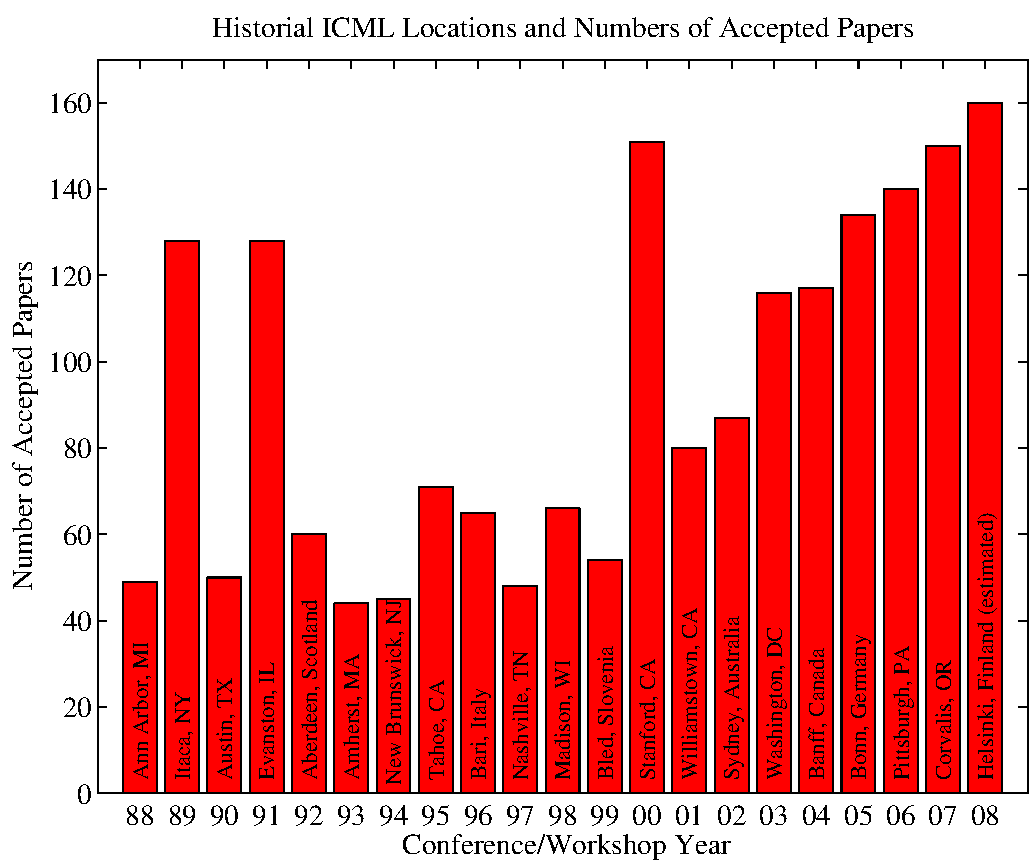
\includegraphics[width=\columnwidth]{icml_numpapers}}
\caption{Historical locations and number of accepted papers for International
  Machine Learning Conferences (ICML 1993 -- ICML 2008) and
  International Workshops on Machine Learning (ML 1988 -- ML
  1992). At the time this figure was produced, the number of
  accepted papers for ICML 2008 was unknown and instead estimated.}
\label{icml-historical}
\end{center}
\vskip -0.2in
\end{figure} 

\subsection{Figures}
 
You may want to include figures in the paper to help readers visualize
your approach and your results. Such artwork should be centered,
legible, and separated from the text. Lines should be dark and at
least 0.5~points thick for purposes of reproduction, and text should
not appear on a gray background.

Label all distinct components of each figure. If the figure takes the
form of a graph, then give a name for each axis and include a legend
that briefly describes each curve. Do not include a title inside the
figure; instead, the caption should serve this function.

Number figures sequentially, placing the figure number and caption
{\it after\/} the graphics, with at least 0.1~inches of space before
the caption and 0.1~inches after it, as in
Figure~\ref{icml-historical}.  The figure caption should be set in
9~point type and centered unless it runs two or more lines, in which
case it should be flush left.  You may float figures to the top or
bottom of a column, and you may set wide figures across both columns
(use the environment {\tt figure*} in \LaTeX), but always place
two-column figures at the top or bottom of the page.

\subsection{Algorithms}

If you are using \LaTeX, please use the ``algorithm'' and ``algorithmic'' 
environments to format pseudocode. These require 
the corresponding stylefiles, algorithm.sty and 
algorithmic.sty, which are supplied with this package. 
Algorithm~\ref{alg:example} shows an example. 

\begin{algorithm}[tb]
   \caption{Bubble Sort}
   \label{alg:example}
\begin{algorithmic}
   \STATE {\bfseries Input:} data $x_i$, size $m$
   \REPEAT
   \STATE Initialize $noChange = true$.
   \FOR{$i=1$ {\bfseries to} $m-1$}
   \IF{$x_i > x_{i+1}$} 
   \STATE Swap $x_i$ and $x_{i+1}$
   \STATE $noChange = false$
   \ENDIF
   \ENDFOR
   \UNTIL{$noChange$ is $true$}
\end{algorithmic}
\end{algorithm}
 
\subsection{Tables} 
 
You may also want to include tables that summarize material. Like 
figures, these should be centered, legible, and numbered consecutively. 
However, place the title {\it above\/} the table with at least 
0.1~inches of space before the title and the same after it, as in 
Table~\ref{sample-table}. The table title should be set in 9~point 
type and centered unless it runs two or more lines, in which case it
should be flush left.

% Note use of \abovespace and \belowspace to get reasonable spacing 
% above and below tabular lines. 

\begin{table}[t]
\caption{Classification accuracies for naive Bayes and flexible 
Bayes on various data sets.}
\label{sample-table}
\vskip 0.15in
\begin{center}
\begin{small}
\begin{sc}
\begin{tabular}{lcccr}
\hline
\abovespace\belowspace
Data set & Naive & Flexible & Better? \\
\hline
\abovespace
Breast    & 95.9$\pm$ 0.2& 96.7$\pm$ 0.2& $\surd$ \\
Cleveland & 83.3$\pm$ 0.6& 80.0$\pm$ 0.6& $\times$\\
Glass2    & 61.9$\pm$ 1.4& 83.8$\pm$ 0.7& $\surd$ \\
Credit    & 74.8$\pm$ 0.5& 78.3$\pm$ 0.6&         \\
Horse     & 73.3$\pm$ 0.9& 69.7$\pm$ 1.0& $\times$\\
Meta      & 67.1$\pm$ 0.6& 76.5$\pm$ 0.5& $\surd$ \\
Pima      & 75.1$\pm$ 0.6& 73.9$\pm$ 0.5&         \\
\belowspace
Vehicle   & 44.9$\pm$ 0.6& 61.5$\pm$ 0.4& $\surd$ \\
\hline
\end{tabular}
\end{sc}
\end{small}
\end{center}
\vskip -0.1in
\end{table}

Tables contain textual material that can be typeset, as contrasted 
with figures, which contain graphical material that must be drawn. 
Specify the contents of each row and column in the table's topmost
row. Again, you may float tables to a column's top or bottom, and set
wide tables across both columns, but place two-column tables at the
top or bottom of the page.
 


% Acknowledgements should only appear in the accepted version. 
\section*{Acknowledgments} 
 
\textbf{Do not} include acknowledgements in the initial version of
the paper submitted for blind review.

If a paper is accepted, the final camera-ready version can (and
probably should) include acknowledgements. In this case, please
place such acknowledgements in an unnumbered section at the
end of the paper. Typically, this will include thanks to reviewers
who gave useful comments, to colleagues who contributed to the ideas, 
and to funding agencies and corporate sponsors that provided financial 
support.  


% In the unusual situation where you want a paper to appear in the
% references without citing it in the main text, use \nocite
%\nocite{langley00}

\bibliography{deep_belief_nets}
\bibliographystyle{icml2013}

\end{document} 


% This document was modified from the file originally made available by
% Pat Langley and Andrea Danyluk for ICML-2K. This version was
% created by Lise Getoor and Tobias Scheffer, it was slightly modified  
% from the 2010 version by Thorsten Joachims & Johannes Fuernkranz, 
% slightly modified from the 2009 version by Kiri Wagstaff and 
% Sam Roweis's 2008 version, which is slightly modified from 
% Prasad Tadepalli's 2007 version which is a lightly 
% changed version of the previous year's version by Andrew Moore, 
% which was in turn edited from those of Kristian Kersting and 
% Codrina Lauth. Alex Smola contributed to the algorithmic style files.  
